% -------------------------------------------------------
%  ___ ___  _ __ ___  _ __   __ _ _ __ ___ 
% / __/ _ \| '_ ` _ \| '_ \ / _` | '__/ _ \
%| (_| (_) | | | | | | |_) | (_| | | |  __/
% \___\___/|_| |_| |_| .__/ \__,_|_|  \___|
%                    |_|                   
% -------------------------------------------------------
\chapter{Models comparison (2-3 pages)}


\section{First Principle Model}
This model \ref{fig:model_equations} was developed with respect to equations
represented before.

\begin{figure}[h!]
    \centering
    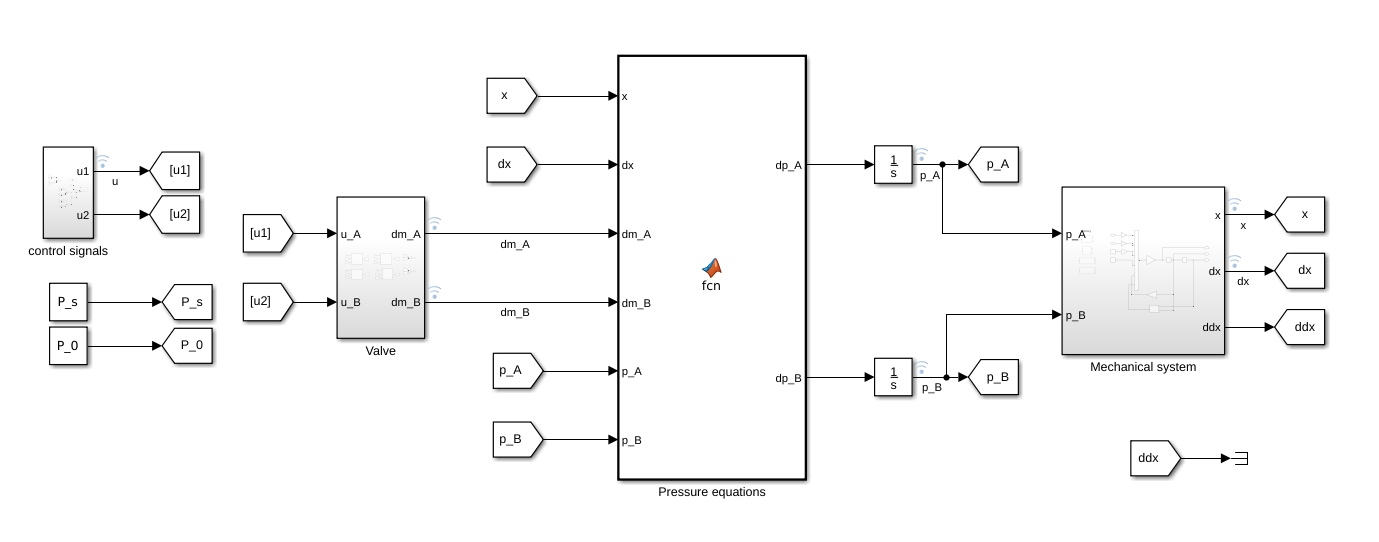
\includegraphics[width=1\textwidth]{equations.png}
    \caption{Simulink model based on equations}
    \label{fig:model_equations}
\end{figure}

\section{Alternative Modeling Techniques (3 pages)}
Generally with dataset of input-output signals approximation model can be
fit. Using System Identification Toolbox and modeled as Black-Box or
Gray-Box models. This section attempted to fit some models using data from
SimScape and Equation model presented before.

Fit approximation model make sense only if we know what to fit. Using
signal process techniques and identify dominant signals that providing best
classification features we will train models with respect to this signals.

\subsection{Physical Model (SimScape)}
Working, very slow. Equations are faster for estimation parameters.
Model \ref{fig:model_simscape} was developed using SimScape toolbox.

\begin{figure}[h!]
    \centering
    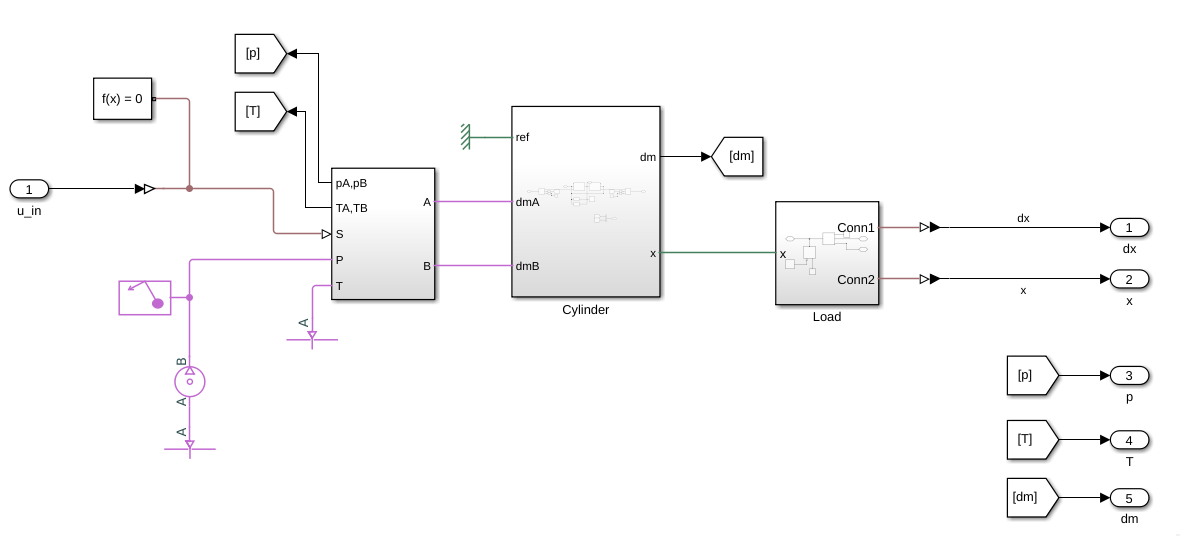
\includegraphics[width=1\textwidth]{simscape.png}
    \caption{Simulink model using SimScape Toolbox}
    \label{fig:model_simscape}
\end{figure}

\subsection{State-space/ARX Models}
Not working, Nonlinearities.


\subsection{Hammerstein-Wiener Model}
Working only for Position.

\subsection{Nonparametric model (ANN)}

Working. Can be used as "Normal operation" model.



\section{Comparison}
Following figure \ref{fig:compare_of_models} represent comparison of 2 models
(Simscape and based on equations) using same parameters for simulation:
There is slight difference between models causing Valve dynamics
simplifications in model based on equations.

\begin{figure}[h!]
    \centering
    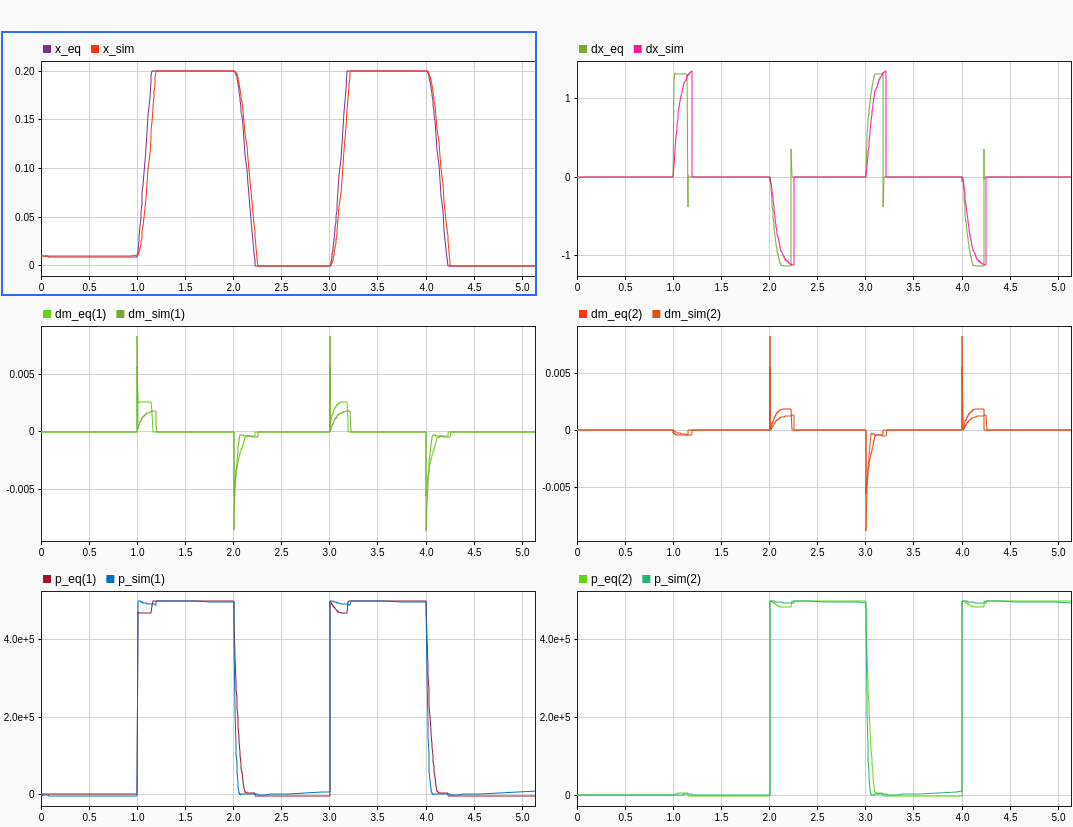
\includegraphics[width=0.8\textwidth]{models_comparation.png}
    \caption{Comparison of simscape and model based on equations}
    \label{fig:compare_of_models}
\end{figure}


